
从并发性的角度来看,\textbf{堆栈}是最简单的数据结构之一。堆栈上的所有操作都处理顶部元素,因此(至少在概念上)需要保护一个位置以防止竞争。

C++标准库提供了\texttt{std::stack}容器,可以将该容器作为一个起点。所有C++容器,都提供了弱线程安全。多个线程可以安全地访问只读容器,只要没有线程调用非\texttt{const}函数,任意数量的线程都可以同时调用任何\texttt{const}方法。这听起来很简单,几乎过于简单,但这里有一个问题。在最后一次修改和只读的部分之间,必须存在某种同步,所有线程在内存栅栏之前执行,写访问并没有真正完成。写线程至少需要释放内存,而读线程必须获取内存。任何强栅栏都可以工作,锁也可以,但每个线程都必须迈出这一步。

\subsubsubsection{7.3.1\hspace{0.2cm}线程安全接口的设计}

现在,如果多个线程在修改堆栈,则需要更强的保证,那该怎么办?提供互斥锁的最直接的方法,用锁保护类的每个成员函数。这可以在应用程序级别完成,但是这样的实现并不是强线程安全,并且很容易出错。因为锁与容器没有关联,也很难进行调试和分析。

更好的选择是用自己的类包装堆栈类:

\hspace*{\fill} \\ %插入空行
\noindent
\textbf{02\_stack.C}
\begin{lstlisting}[style=styleCXX]
template <typename T> class mt_stack {
	std::stack<T> s_;
	std::mutex l_;
	public:
	mt_stack() = default;
	void push(const T& v) {
		std::lock_guard g(l_);
		s_.push(v);
	}
	…
};
\end{lstlisting}

注意,可以使用继承而不是封装。这样做会使\texttt{mt\_stack}的构造函数更简单,只需要一个\texttt{using}语句。但是,使用公共继承会公开基类\texttt{std::stack}的每个成员函数,若忘记包装其中一个,代码将直接调用未保护的成员函数。私有(或受保护的)继承避免了这个问题,但会带来其他风险。有些构造函数需要重新实现,例如:移动构造函数需要锁定正在移动的堆栈,因此需要自定义实现。在没有包装器的情况下,公开其他几个构造函数十分危险,因为它们会读取或修改参数。总的来说,必须重写每个构造函数,这样比较安全。这与C++的建议是一致的,\textit{组合优于继承}(\textit{prefer composition over inheritance})。

线程安全或多线程堆栈(就是\textit{mt}的意思)现在有了\textit{push}功能,并准备接收数据。现在,只需要逆操作\textit{pop}。当然可以按照前面的例子包装\texttt{pop()},但这还远远不够。STL堆栈使用三个独立的成员函数从堆栈中删除元素,\texttt{pop()}删除了顶部元素,但没有任何返回。所以想知道堆栈顶部是什么,必须先使用\texttt{top()}。如果堆栈为空,那么使用这两种方法中的任何一个都会导致未定义行为,所以必须先使用\texttt{empty()}检查结果。这里需要包装这三个方法,这里先不展示。下面的代码中,假设堆栈的所有成员函数都由一个锁保护:

\begin{lstlisting}[style=styleCXX]
mt_stack<int> s;
… push some data on the stack …
int x = 0;
if (!s.empty()) {
	x = s.top();
	s.pop();
}
\end{lstlisting}

每个成员函数都是线程安全的,但在多线程上下文中完全没用。堆栈可能在某一刻(碰巧使用\texttt{s.empty()}的那一刻)非空,但在下一刻(调用\texttt{s.top()}之前)就变成空的了,在此期间另一个线程可以删除顶部的元素。

这可能是整本书最重要的内容了。为了提供可用的线程安全功能,在选择接口时必须考虑线程安全,但不能在现有的设计上添加线程安全的特性。在进行设计时,必须考虑到线程安全。因为可以选择在设计中提供某些保证和不变量,这些在并发程序中不可维护,例如:\texttt{std::stack}保证调用\texttt{empty()}是安全的,并返回false,这样就可以安全地调用\texttt{top()},只要在这两个调用间不做其他的堆栈操作就好。在多线程程序中,没有特别好的方法来履行这种承诺。

幸运的是,由于正在编写自己的包装器类,所以不需要逐个使用包装类的接口。那么,应该怎么做呢?显然,整个\texttt{pop}操作是一个成员函数,应该从堆栈中删除顶部元素,并将其返回给调用者。问题是当堆栈为空时该做什么?有多种选择。可以返回一对值和一个布尔标志,该标志指示堆栈是否为空(这种情况下,该值必须有默认构造)。也可以单独返回布尔值,并通过引用传递该值(如果堆栈为空,则该值保持不变)。在C++17中,解决方案是返回\texttt{std::optional},如以下代码所示。它非常适合持有可能并不存在的值:

\hspace*{\fill} \\ %插入空行
\noindent
\textbf{02\_stack.C}
\begin{lstlisting}[style=styleCXX]
template <typename T> class mt_stack {
	std::stack<T> s_;
	std::mutex l_;
	public:
	std::optional<T> pop() {
		std::lock_guard g(l_);
		if (s_.empty()) {
			return std::optional<T>(std::nullopt);
		} else {
			std::optional<T> res(std::move(s_.top()));
			s_.pop();
			return res;
		}
	}
};
\end{lstlisting}

将元素从堆栈中弹出的整个操作现在都受到锁的保护,这个接口是事务性的。每个成员函数将对象从一个已知状态转到另一个已知状态。

如果对象必须转换到一些中间状态,比如使用\texttt{empty()}之后,并在使用\texttt{pop()}之前的状态,这些状态必须对使用者不可见。相反,向使用者呈现的是原子事务。要么返回顶部的元素,要么通知调用者不能进行该操作,这确保了程序的正确性。现在,来看看性能。

\subsubsubsection{7.3.2\hspace{0.2cm}使用互斥的性能}

堆栈的性能如何?假设每个操作从开始到结束都是锁定的,那就不要对堆栈成员函数的性能有什么期待。最好的情况下线程都将串行地执行堆栈操作,实际中锁应该会带来一些额外的开销。如果要比较多线程堆栈和普通\texttt{std::stack}的性能,可以在基准测试中进行对比。

为了简化基准测试,可以选择在\texttt{std::stack}上实现单线程的非阻塞包装器,该包装器提供与\texttt{mt\_stack}相同的接口。注意,不能仅通过\texttt{push}堆栈来进行基准测试,这样基准测试可能会将内存耗尽。类似地,无法可靠地对\texttt{pop}操作进行基准测试,除非想测量从空堆栈弹出的耗时。如果基准测试运行的时间足够长,就必须将\texttt{push}和\texttt{pop}结合起来。最简单的基准测试可以是这样的:

\hspace*{\fill} \\ %插入空行
\noindent
\textbf{02\_stack.C}
\begin{lstlisting}[style=styleCXX]
mt_stack<int> s;
void BM_stack(benchmark::State& state) {
	const size_t N = state.range(0);
	for (auto _ : state) {
		for (size_t i = 0; i < N; ++i) s.push(i);
		for (size_t i = 0; i < N; ++i)
		benchmark::DoNotOptimize(s.pop());
	}
	state.SetItemsProcessed(state.iterations()*N);
}
\end{lstlisting}

多线程时,有可能在堆栈为空时进行\texttt{pop()}操作。对于处于设计阶段的堆栈来说,这是可能现实的。此外,由于基准测试提供了真实应用程序中数据结构性能的近似值,其中的差异可以忽略。不过,为了获得更精确的测量值,必须模拟应用程序,并执行真实的\texttt{push}和\texttt{pop}操作序列。结果应该是这样的:

%\hspace*{\fill} \\ %插入空行
\begin{center}
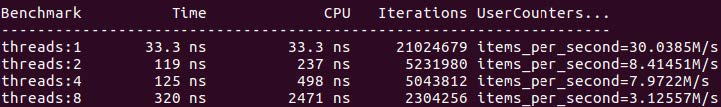
\includegraphics[width=0.9\textwidth]{content/2/chapter7/images/3.jpg}\\
图7.3 - 锁栈——使用互斥锁——的性能
\end{center}

注意这里的“item”是“push后面跟着pop”的操作,所以“items per second”的值显示了每秒钟可以通过堆栈发送多少数据。为了进行比较,没有锁的堆栈在单个线程上的执行速度,要比使用互斥锁快10倍多:

%\hspace*{\fill} \\ %插入空行
\begin{center}
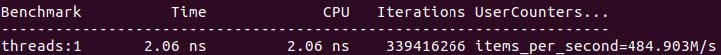
\includegraphics[width=0.9\textwidth]{content/2/chapter7/images/4.jpg}\\
图7.4 - \texttt{std::stack}的性能(与图7.3相比)
\end{center}

使用互斥对象实现的堆栈性能相当差。但不要急于设计一些聪明的线程安全堆栈,现在还不需要。这时,应该问的第一个问题是,这是怎么回事?应用程序如何处理堆栈上的数据?如果每个数据元素都需要耗时几秒钟模拟一个参数,那么堆栈的速度就不重要了。另外,如果堆栈位于某些实时事务处理系统的核心,那么其速度可能是整个系统性能的关键。

顺便说一下,结果可能与其他数据结构类似,如链表、双端队列、队列和树。其中,单个操作要比对互斥锁的操作快得多。但是,在尝试改进性能之前,必须准确地了解应用程序需要什么样的性能。

\subsubsubsection{7.3.3\hspace{0.2cm}不同的性能需求}

本章的其余部分中,假设数据结构的性能在应用程序中很重要。现在,可以来聊聊最快的堆栈实现了吧?还没到那个时候。还需要考虑使用的模型,该如何处理堆栈,以及什么才是需要加速的东西。

互斥锁堆栈性能较差的关键原因是,速度基本上受到互斥锁的限制,对堆栈操作进行基准测试几乎与对互斥锁的锁定和解锁进行基准测试结果相同。提高性能的一种方法是改进互斥锁的实现,或者使用另一种同步方案。另一种方法是少使用互斥锁,这需要重新设计客户端代码。

例如,使用者通常有多个必须压入堆栈的项。类似地,使用者可以一次从堆栈中弹出几个元素并进行处理。这种情况下,可以使用数组或容器来实现批量推送或批量弹出,以便一次从堆栈中复制多个元素。由于锁定的开销很大,可以用锁定/解锁操作在堆栈上一次性推入1024个元素,这样就比用锁逐个推入元素来的快,基准测试也反映了这一点:

%\hspace*{\fill} \\ %插入空行
\begin{center}
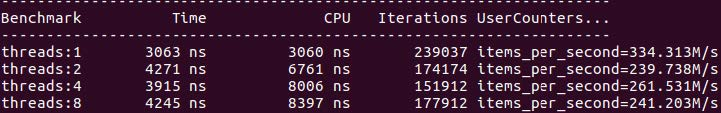
\includegraphics[width=0.9\textwidth]{content/2/chapter7/images/5.jpg}\\
图7.5 - 批处理堆栈操作的性能(每个锁1024个元素)
\end{center}

我们应该非常清楚这种方式可以做哪些事,不能做哪些事。若临界区内的操作比锁操作本身快得多,就该减少锁的开销,但不能锁定操作的规模。此外,通过延长停留在临界区的时间,迫使线程在锁上等待更长时间。如果所有线程都尝试访问堆栈(这就是基准测试变得更快的原因),那没问题。但若在应用程序中,线程主要是执行其他计算,只是偶尔访问堆栈,那么较长的等待可能会降低整体性能。为了明确地回答批量\texttt{push}和批量\texttt{pop}是否对性能有益,必须在更真实的环境中进行分析。

其他一些场景中,寻找更有限的、特定于应用程序的解决方案,可以获得远高于通用解决方案的改进,从而获得的性能收益。单个线程将大量数据提前\texttt{push}到堆栈上,然后多个线程将数据从堆栈中删除并处理,可能还会将更多数据\texttt{push}到堆栈上。这种情况可以实现解锁的\texttt{push},只在单线程中的\texttt{push}中使用。虽然使用者的责任是,永远不要在多线程中使用这个方法,但解锁的堆栈比锁定的堆栈快得多,因此这里的复杂性是值得的。

更复杂的数据结构提供了各种各样的使用模型,但即使是堆栈也可以使用,而不仅仅是简单的\texttt{push}和\texttt{pop}。也可以查看顶部的元素而不删除,\texttt{std::stack}提供了\texttt{top()}成员函数,但不是事务性的,所以必须创建自己的函数。其非常类似于事务性的\texttt{pop()}函数,只是不移除顶部的元素:

\hspace*{\fill} \\ %插入空行
\noindent
\textbf{02\_stack.C}
\begin{lstlisting}[style=styleCXX]
template <typename T> class mt_stack {
	std::stack<T> s_;
	mutable std::mutex l_;
	public:
	std::optional<T> top() const {
		std::lock_guard g(l_);
		if (s_.empty()) {
			return std::optional<T>(std::nullopt);
		} else {
			std::optional<T> res(s_.top());
			return res;
		}
	}
};
\end{lstlisting}

注意,为了允许只进行查找,这里\texttt{top()}声明为\texttt{const},这里必须将互斥量声明为\texttt{mutable}。这样做时要小心,多线程程序的约定是遵循STL,只要不调用非\texttt{const}成员函数,所有\texttt{const}成员函数都可以安全地在多个线程上使用。这意味着\texttt{const}函数不会修改只读对象,而可变数据成员违背了这个假设。至少,不应该表示对象的逻辑状态。然后,在修改时应该避免竞争条件。互斥锁必须满足这两个要求。

现在可以考虑不同的使用模式。某些应用程序中,数据\texttt{push}入堆栈,再从中\texttt{pop}出。其他情况下,堆顶元素可能需要在每次\texttt{push}和\texttt{pop}之间检查多次。先关注后一种情况,而后再次检查\texttt{top()}。这里有一个明显的低效行为,由于锁的存在,只有一个线程可以读取栈顶元素。但是读取栈顶元素是一个非修改(只读)操作。如果所有线程都这样做,并且没有线程同时尝试修改堆栈,那么就不需要锁。但现在,它的性能与\texttt{pop()}一样。

不能在\texttt{top()}中省略锁,原因是不能确定另一个线程在同一时间没有使用\texttt{push()}或\texttt{pop()}。但即使这样,也不需要对\texttt{top()}进行两次锁定,它们可以同时进行,只有修改堆栈的操作需要锁定。有一种类型的锁提供这样的功能,称为\textbf{读写锁}。任何数量的线程都可以获得读锁,并且这些线程之间不会互相影响。但是,写锁只能由一个线程获得,而且只有在没有其他线程持有读锁的情况下才能获取。在C++中,术语不同(但功能完全相同),读线程使用共享锁(同一个互斥对象上的共享锁可以同时存在),但写线程需要唯一锁(给定的互斥对象上只能存在一个这样的锁)。如果另一个线程已经持有唯一锁,那么获取共享锁的尝试将会阻塞。同样,若另一个线程持有同一个互斥对象上的锁,那么获取唯一锁的尝试将会阻塞。有了共享互斥锁,就可以用需要的那种锁来实现堆栈。\texttt{top()}使用了共享锁后,任意数量的线程都可以同时执行,但\texttt{push()}和\texttt{pop()}需要唯一锁:

\begin{lstlisting}[style=styleCXX]
template <typename T> class rw_stack {
	std::stack<T> s_;
	mutable std::shared_mutex l_;
	public:
	void push(const T& v) {
		std::unique_lock g(l_);
		s_.push(v);
	}
	std::optional<T> pop() {
		std::unique_lock g(l_);
		if (s_.empty()) {
			return std::optional<T>(std::nullopt);
		} else {
			std::optional<T> res(std::move(s_.top()));
			s_.pop();
			return res;
		}
	}
	std::optional<T> top() const {
		std::shared_lock g(l_);
		if (s_.empty()) {
			return std::optional<T>(std::nullopt);
		} else {
			std::optional<T> res(s_.top());
			return res;
		}
	}
};
\end{lstlisting}

但基准测试显示,使用\texttt{top()}的性能即使在读写锁下也不会改变:

%\hspace*{\fill} \\ %插入空行
\begin{center}
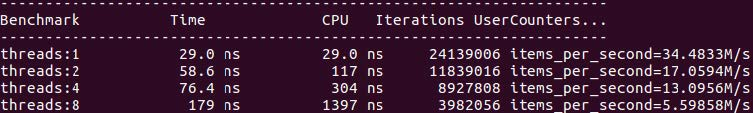
\includegraphics[width=0.9\textwidth]{content/2/chapter7/images/6.jpg}\\
图7.6 - 使用\texttt{std::shared\_mutex}栈的性能——只读操作
\end{center}

与普通互斥锁相比,唯一锁的性能下降得更厉害:

%\hspace*{\fill} \\ %插入空行
\begin{center}
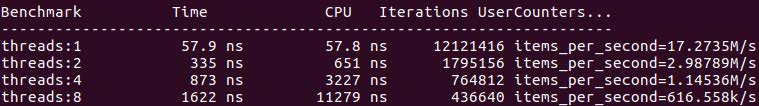
\includegraphics[width=0.9\textwidth]{content/2/chapter7/images/7.jpg}\\
图7.7 - 使用\texttt{std::shared\_mutex}栈的性能——写入操作
\end{center}

将图7.6和7.7与图7.4中的测试值进行比较,可以看到读写锁并没有任何改进。这个结论并不普遍,因为不同互斥量的性能取决于实现和硬件。然而,更复杂的锁,比如共享互斥锁,会比简单锁有更多的开销。它们的目标程序不同的,若临界区内的操作花费的时间非常久多(比如,毫秒而不是微秒),并且大多数线程执行只读代码,那么就没必要锁定只读线程将。

观察更长的临界段是非常重要的。如果堆栈元素较大,并且复制的代价非常高,那么与复制大对象的代价相比,锁的性能就不重要了。假设总体目标是使程序快速,而不是展示可扩展的堆栈实现,这里将通过消除昂贵的复制,并使用指针堆栈来优化整个应用程序。

尽管读写锁遇到了挫折,但我们正确的走在实现更高效应用的路上。在进行设计之前,我们必须更详细地了解每个堆栈操作的作用,以及在每个步骤中必须避免可能出现的数据竞争。

\subsubsubsection{7.3.4\hspace{0.2cm}堆栈性能详情}

在尝试提高线程安全堆栈(或其他数据结构)的性能(不是简单的锁保护实现)时,必须详细了解每个操作所涉及的步骤,以及如何与在不同线程上与其他操作交互。本节的目标不是更快的堆栈,而是进行分析。因为底层步骤在许多数据结构中都有,这里我们从\texttt{push}操作开始。大多数堆栈实现都是建立在类似数组的容器上,所以可以把堆栈的顶部看作是一个连续的内存块:

%\hspace*{\fill} \\ %插入空行
\begin{center}
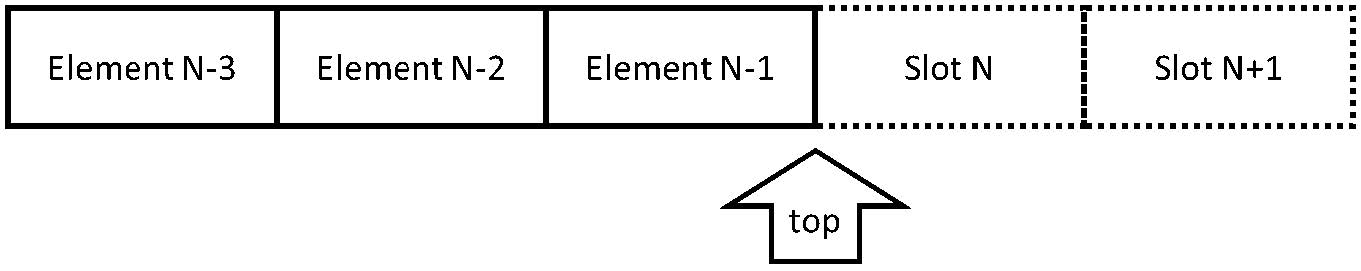
\includegraphics[width=0.9\textwidth]{content/2/chapter7/images/8.jpg}\\
图7.8 - 栈顶的\texttt{push}操作
\end{center}

堆栈上有N个元素,所以元素计数也是下一个元素的槽索引。\texttt{push}操作必须将\texttt{top}索引(也是元素计数)从N增加到N+1,以保留槽位,然后在槽位N中构造新元素。注意,这个\texttt{top}索引是执行\texttt{push}操作的线程。只要索引增量操作是线程安全的,那么只有一个线程可以看到索引的值。执行\texttt{push}操作的第一个线程将顶部索引提升到N+1,并保留第N个槽位,下一个线程将索引增加到N+2,并保留第N+1个槽位,以此类推。这里的关键是插槽不存在竞争,因为只有一个线程可以获得特定的插槽,因此可以在那里构造对象,而不会有其他线程进行干扰。

这就为\texttt{push}操作提供了非常简单的同步方案,所需要的只是栈顶索引是原子值:

\begin{lstlisting}[style=styleCXX]
std::atomic<size_t> top_;
\end{lstlisting}

\texttt{push}操作会自动增加这个索引,然后在数组槽中构造新元素(按索引的旧值索引):

\begin{lstlisting}[style=styleCXX]
const size_t top = top_.fetch_add(1);
new (&data[top]) Element(… constructor arguments … );
\end{lstlisting}

同样,不需要保护构造步骤。要让\texttt{push}操作线程安全,只需要原子索引即可。如果使用数组作为堆栈内存,也没问题。若使用\texttt{std::deque}这样的容器,就不能简单地在内存上构造一个新元素了,这里需要使用\texttt{push\_back}来更新容器,而且这个操作不是线程安全的,即\texttt{deque}可能不需要分配更多的内存。由于这个原因,不在锁管理下数据结构通常需要自己管理内存。说到内存,到目前为止,我们假设数组有足够的空间添加更多的元素,并且不会耗尽内存。这里继续坚持这个假设。

现在,在特定情况下实现线程安全的\texttt{push}操作,是一种非常高效的方式。多个线程会将数据推送到堆栈上,但在所有的\texttt{push}操作完成之前不能读取数据。

若有一个堆栈,其中已经有了元素,需要弹出它们(并且没有添加更多的新元素),也可以使用相同的方法。图7.8也适用于这种场景:一个线程自动减少\texttt{top}计数,然后返回\texttt{top}元素:

\begin{lstlisting}[style=styleCXX]
const size_t top = top_.fetch_sub(1);
return std::move(data[top]);
\end{lstlisting}

原子自减保证了只有一个线程可以访问顶部元素的数组槽。当然,这只在堆栈不是空的情况下才有效。可以将顶部元素的索引从无符号改为有符号整数,当索引为负时,就知道堆栈为空了。

这也是在非常特殊的条件下,实现线程安全\texttt{pop}操作的一种有效方式。堆栈已经填充,并且没有添加新元素。本例中,还需要知道堆栈上有多少元素,因此可以避免弹出空堆栈。

一些特定的应用程序中,这可能是有价值的。若堆栈由多个线程填充,没有任何弹出,并且在程序中有明确定义的点,从添加数据切换到删除数据,就存在一个很好的解决方案。不过,现在我们想继续讨论更一般的情况。

但高效的\texttt{push}操作对于从栈中读取数据毫无帮助,需要考虑如何实现弹出顶部元素的操作。我们有顶部索引,但它只表明当前有多少元素正在构造。没有提到构造最后一个元素的位置(图7.9中的元素N-3):

%\hspace*{\fill} \\ %插入空行
\begin{center}
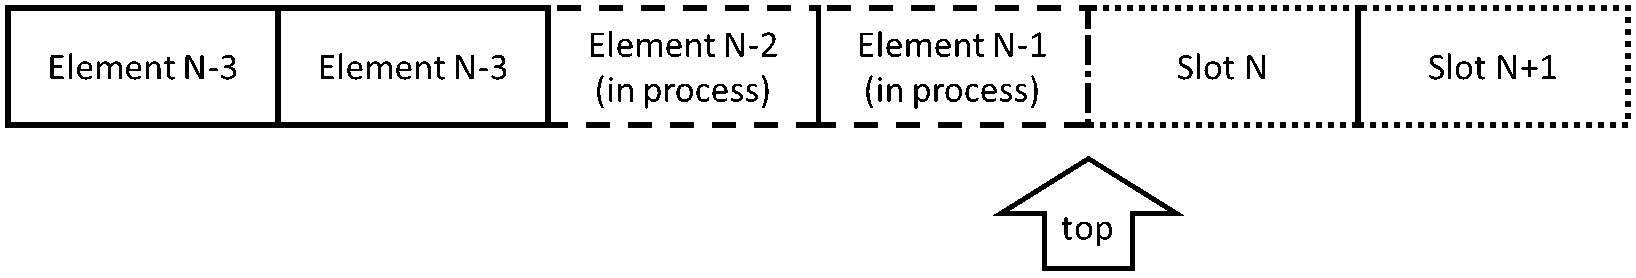
\includegraphics[width=0.9\textwidth]{content/2/chapter7/images/9.jpg}\\
图7.9 - \texttt{push}和\texttt{pop}操作栈的顶部
\end{center}

当然,执行\texttt{push}和构造操作的线程,知道什么时候完成构造。也许需要的是另一个计数,显示有多少元素完成构造。唉……要是有那么简单就好了。图7.9中,假设线程A正在构造元素N-2,而线程B正在构造元素N-1。显然,线程A是第一个增加顶索引的。但这并不意味着它也是第一个完成\texttt{push}操作的,也许线程B可以先完成构造。现在,堆栈上最后一个构造元素的索引是N-1,所以可以将构造计数提升到N-1(注意,跳过了仍在构造中的元素N-2)。现在想要弹出顶部元素。没问题,因为元素N-1已经准备好了,所以可以把它返回给使用者,并从堆栈中移除,构造计数现在减少到N-2。接下来应该弹出哪个元素?元素N-2没有准备好,但堆栈中没有任何警告。只有一个完成元素的计数,它的值是N-1。现在,在堆栈上构造新元素的线程和试图弹出新元素的线程之间,出现了数据竞争。

即使没有竞争,还有另一个问题:只弹出元素N-1,这在当时是正确的做法。但是,当线程C请求了一个\texttt{push}时,应该使用哪个插槽?如果使用槽位N-1,则可能会覆盖线程A当前访问的元素。如果使用槽位N,当所有的操作都完成,数组中就会出现一个洞。顶部的元素是N,但下一个元素不是N-1,N-1已经弹出,必须跳过它。据结构没有告诉我们必须这样做。

可以跟踪哪些元素是存在,哪些元素是洞,但这些问题会将场面弄得越来越复杂(以线程安全的方式进行将需要额外的同步,这会降低性能)。另外,留下许多未使用的数组槽会浪费内存。可以尝试为\texttt{push}堆栈的新元素重用已空闲的槽,但这时元素不再连续存储,原子顶部计数不再工作,整个结构类似于一个链表。如果认为链表是实现线程安全堆栈的好方法,在本章后面的内容中会看到如何实现线程安全的链表。

在设计上,必须暂停深入研究实现细节,并再次检查解决问题的更一般方法。需要由两个步骤完成:从对堆栈实现细节的更深入理解中总结出结论,并进行性能估计,以大致了解哪些解决方案可能会带来性能上的改进。我们先从后者开始。

\subsubsubsection{7.3.5\hspace{0.2cm}同步方案的性能评估}

我们第一次尝试在没有锁的情况下实现一个堆栈,也产生了一些有趣的解决方案,但并没有通用的解决方案。在花更多的时间构建一个复杂的设计之前,应该试着评估其比基于锁的设计,更有效率的可能性有多大。

当然,这看起来像是循环推理。为了估计性能,必须首先对一些东西进行评估。但是我们不想浪费时间进行复杂的设计,所以才需要进行性能评估。

幸运的是,我们可以参考前面观察的结果。并发数据结构的性能,很大程度上取决于并发访问多少共享变量。假设可以想出一种聪明的方法,用一个原子计数器来实现堆栈。可以合理地假设,每次\texttt{push}和\texttt{pop}都必须对这个计数器进行至少一次原子递增或递减操作(除非正在进行批处理操作)。如果将单线程堆栈上的\texttt{push}和\texttt{pop}与共享原子计数器上的原子操作结合起来进行基准测试,可以得到一个合理的性能评估。因为没有同步,所以必须为每个线程使用单独的堆栈,以避免条件竞争:

\begin{lstlisting}[style=styleCXX]
std::atomic<size_t> n;
void BM_stack0_inc(benchmark::State& state) {
	st_stack<int> s0;
	const size_t N = state.range(0);
	for (auto _ : state) {
		for (size_t i = 0; i < N; ++i) {
			n.fetch_add(1, std::memory_order_release);
			s0.push(i);
		}
		for (size_t i = 0; i < N; ++i) {
			n.fetch_sub(1, std::memory_order_acquire);
			benchmark::DoNotOptimize(s0.pop());
		}
	}
	state.SetItemsProcessed(state.iterations()*N);
}
\end{lstlisting}

\texttt{st\_stack}是堆栈包装器,提供的接口与基于锁的\texttt{mt\_stack}相同,但不使用锁。实际表现会稍微慢一些,因为堆栈顶部在线程之间共享,但这将会是对上面实现的评估:任何真正线程安全的实现,都不太可能比这个基准测试的性能更好。那用什么来比较结果呢?图7.3中基于锁的堆栈基准展示了堆栈的性能,在线程上每秒进行30M次\texttt{push/pop}操作,在8个线程上每秒进行3.1M的\texttt{push/pop}操作。在没有锁的情况下,堆栈的基线性能大约是每秒\texttt{485M}个操作(图7.4)。在同一台机器上,使用单个原子计数器进行性能评估,结果如下:

%\hspace*{\fill} \\ %插入空行
\begin{center}
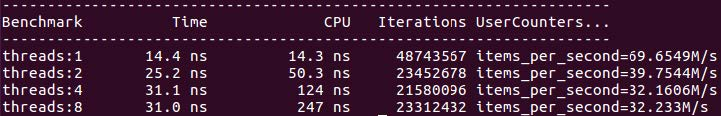
\includegraphics[width=0.9\textwidth]{content/2/chapter7/images/10.jpg}\\
图7.10 - 性能评估——使用单个原子计数器的堆栈
\end{center}

结果看起来很复杂。即使在最优条件下,堆栈性能也不会改变。同样,这主要是因为测试的是一堆小元素。因为多个线程可以同时复制数据,如果元素很大,且复制成本很高,就会看到扩展的性能。如果复制数据变得非常昂贵,需要很多线程来完成它,最好使用指针堆栈,从而不用复制任何数据。

另一方面,原子计数器要比基于互斥锁的堆栈快得多。当然,这是上面的评估,但它表明无锁堆栈存在一些可能性。然而,基于锁的堆栈也是如此。当需要锁定非常小的临界区时,有比\texttt{std::mutex}更高效的锁。实现自旋锁后(已经在第6章中看到过一个这样的锁),并在基于锁的堆栈中使用这个自旋锁,与图7.2不同,会得到如下的结果:

%\hspace*{\fill} \\ %插入空行
\begin{center}
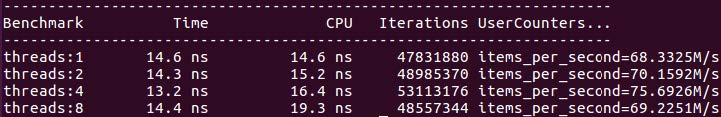
\includegraphics[width=0.9\textwidth]{content/2/chapter7/images/11.jpg}\\
图7.11 - 基于自旋锁堆栈的性能
\end{center}

将这个结果与图7.10进行比较,会得出非常令人沮丧的结果,我们已经想不出一个比简单自旋锁更好的无锁设计。某些情况下,自旋锁的性能优于原子增量的原因,与不同的原子指令在特定硬件上的相对性能有关。所以这里,不应该对此过度解读。

可以尝试用原子交换或比较-交换代替原子增量来完成评估测试。随着了解了更多关于设计线程安全数据结构的知识,还将了解到有哪些同步协议可能有用,以及应该在评估中加入哪些操作。此外,如果使用特定的硬件,应该运行简单的基准来确定哪些操作在该硬件上更高效。目前,所有的结果都是在基于x86的硬件上获得的。如果在专门为HPC应用程序设计的基于ARM的大型服务器上运行相同的评估测试,会得到非常不同的结果。基于锁的堆栈的基准测试结果如下所示:

%\hspace*{\fill} \\ %插入空行
\begin{center}
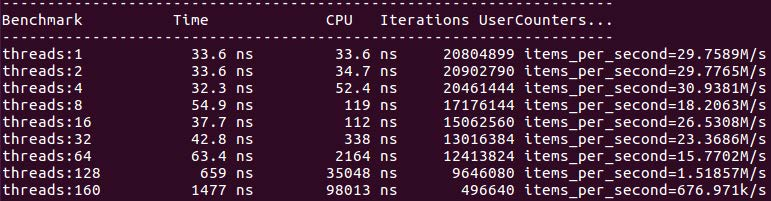
\includegraphics[width=0.9\textwidth]{content/2/chapter7/images/12.jpg}\\
图7.12 - 基于锁的堆栈在ARM HPC系统上的性能
\end{center}

ARM系统通常比x86系统有更多的内核,而单个内核的性能较低。这个特定系统的两个物理处理器上有160个核,当程序在两个CPU上运行时,锁的性能会显著下降。对无锁堆栈性能上限的评估应该使用比较-交换指令来完成,而不是使用原子增量(后者在这些处理器上的效率特别低)。

\hspace*{\fill} \\ %插入空行
\begin{center}
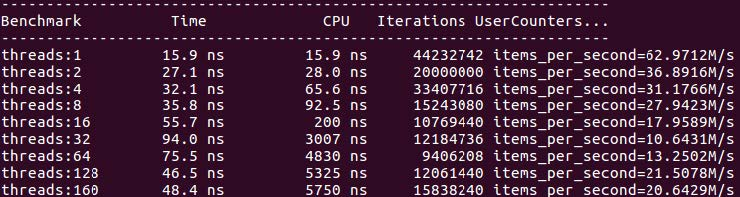
\includegraphics[width=0.9\textwidth]{content/2/chapter7/images/13.jpg}\\
图7.13 - 堆栈中CAS操作的性能评估(ARM处理器)
\end{center}

根据图7.13中的评估,对于大量的线程,可能有比基于锁的堆栈更好的方法。我们将继续努力开发一个无锁堆栈,原因有二:首先,这种努力最终会在某些硬件上得到回报。其次,这个设计的基本元素将在许多其他数据结构中看到,并且堆栈可以提供了一个简单的测试用例进行学习。

\subsubsubsection{7.3.6\hspace{0.2cm}无锁的堆栈}

既然已经决定尝试,并超越一个简单的基于锁的实现,需要考虑一下从\texttt{push}和\texttt{pop}操作本身的探索中获得的经验。每一个操作都很简单,但两者的交叉使用考究增加了复杂性。在多个线程上正确地同步生产者和消费者操作,要比只处理生产者或消费者操作困难得多。在设计自己的数据结构时请牢记,若应用程序允许对需要支持的操作进行类型限制,例如生产者和消费者在时间上是分开的,或者有一个生产者(或消费者)线程,那么肯定可以为这些有限的操作,设计一个更快的数据结构。

假设需要一个完全通用的堆栈,生产者-消费者交互问题的本质可以通过一个简单的例子来理解。同样,假设堆栈是在数组或类似数组的容器之上实现,并且元素是连续存储。假设堆栈上现在有N个元素,生产者线程P正在执行\texttt{push}操作,同时消费者线程C正在执行\texttt{pop}操作。结果是什么?虽然很想尝试一种无等待的设计(就像为仅消费者或仅生产者所做的那样),但允许两个线程在不等待的情况下进行的设计,都将打破对于元素如何存储的假设。线程C必须等待线程P完成\texttt{push}操作,或者返回当前的顶部元素N。类似地,线程P必须等待线程C完成\texttt{push}操作,或者在槽N+1中构造一个新元素。如果两个线程都没有等待,那数组中就会出现空洞。最后一个元素的索引是N+1,但槽位N中没有存储任何内容,所以当从堆栈中弹出数据时,必须以某种方式跳过它。

看起来必须放弃无等待堆栈实现的想法,让其中一个线程等待另一个线程完成它的操作。还必须处理当顶部索引为0,且消费者线程试图进一步减少它时堆栈为空的可能性。当顶部索引指向最后一个元素时,数组的上界也会出现类似的问题,而生产者线程需要另一个槽。

这两个问题都需要一个有界的原子自增操作。除非值等于指定值,才进行自增(或自减)。在C++中(或主流硬件上)没有现成的原子操作,可以使用比较-交换(CAS)来实现,如下所示:

\begin{lstlisting}[style=styleCXX]
std::atomic<int> n_ = 0;
int bounded_fetch_add(int dn, int maxn) {
	int n = n_.load(std::memory_order_relaxed);
	do {
		if (n + dn >= maxn || n + dn < 0) return -1;
	} while (!n_.compare_exchange_weak(n, n + dn,
			std::memory_order_release,
			std::memory_order_relaxed));
	return n;
}
\end{lstlisting}

这是一个非常典型的例子,说明如何使用CAS操作实现一个复杂的无锁原子操作:

\begin{enumerate}
\item 读取变量的当前值。
\item 检查必要的条件。本例中,验证了增量不会给指定边界外的值[0, maxn]。如果有界增量失败,返回-1(通常,对于越界的情况,需要执行特定的操作)。
\item 如果当前值等于前面读取的值,则会原子地将该值替换为所需的结果。
\item 如果步骤3失败,则当前值已更新,请再次检查它,并重复步骤3和4,直到成功。
\end{enumerate}

虽然这看起来像是一种锁,但与锁有一个根本的区别:CAS比较在一个线程上失败的唯一原因是它在另一个线程上成功了(并且原子变量增加了),所以出现共享资源争用时,至少有一个线程可以成功。

还有一个更重要的观察结论,它常常决定了可扩展的实现和低效的实现之间的差别。CAS循环对大多数现代操作系统的调度算法非常不利,不能成功循环的线程会消耗更多的CPU时间,并将赋予更高的优先级。这与想要的完全相反,希望当前正在做有用工作的线程运行得更快。解决方案是让一个线程在尝试了几次不成功的CAS之后生成调度,这可以通过系统调用来完成,但是C++有一个系统独立的API,可以通过\texttt{std::this\_thread::yield()}进行。在Linux上,可以通过每隔几次循环调用\texttt{nanosleep()}进行休眠,从而获得尽可能短的时间(1纳秒)来获得更好的性能:

\begin{lstlisting}[style=styleCXX]
int i = 0;
while ( … ) {
	if (++i == 8) {
		static constexpr timespec ns = { 0, 1 };
		i = 0;
		nanosleep(&ns, NULL);
	}
}
\end{lstlisting}

同样的方法也可以用于实现更复杂的原子事务,比如堆栈\texttt{push}和\texttt{pop},但必须先弄清楚需要哪些原子变量。对于生产者线程,需要数组中第一个空闲槽的索引。对于消费者线程,需要最后一个完成构造的元素的索引。这需要堆栈当前状态的信息,并不允许数组中有“洞”出现:

%\hspace*{\fill} \\ %插入空行
\begin{center}
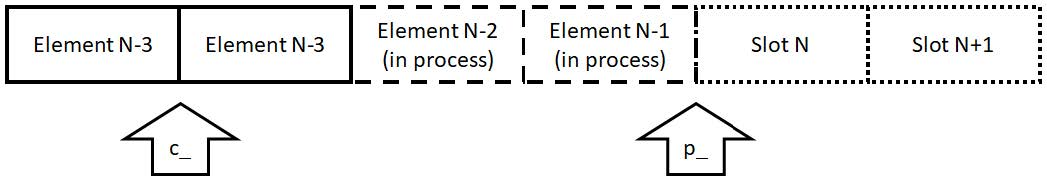
\includegraphics[width=0.9\textwidth]{content/2/chapter7/images/14.jpg}\\ 
图7.14 —— 无锁堆栈:\texttt{c\_}是最后一个完成构造的元素的索引,\texttt{p\_}是数组中第一个空闲槽的索引
\end{center}

如果两个索引当前不相等,\texttt{push}和\texttt{pop}都不能进行。不同的计数意味着要么构造一个新元素,要么是复制当前顶部元素。在这种状态下的堆栈修改都可能导致数组中出现空洞。

如果两个索引相等,就可以继续。为了执行\texttt{push}操作,需要自动增加生产者索引\texttt{p\_}(受数组当前容量限制)。然后,可以在刚才保留的槽中构造新元素(以旧的\texttt{p\_}值为索引)。然后,增加消费者索引\texttt{c\_},表示新元素对消费者线程可用。注意,另一个生产者线程可以在构造完成之前获取下一个插槽,但必须等到所有新元素都构造好之后,才允许消费者线程弹出元素。这样的实现是可能的,但更复杂,而且倾向于当前执行的操作。如果当前正在进行\texttt{push},则\texttt{pop}必须等待,但另一个\texttt{push}可以立即进行。结果很可能是,当所有消费者线程都在等待时,一堆\texttt{push}操作正在执行(如果\texttt{pop}操作正在进行,效果类似)。

\texttt{pop}的实现与此类似,只是首先递减消费索引\texttt{c\_}以保留顶部的位置,然后递减\texttt{p\_}从堆栈中复制或移动对象。

还需要学习一个技巧,那就是如何在原子上处理这两个数。例如,线程必须等待两个索引值相等,如何做到?如果以原子的方式读取一个索引,然后以原子的方式读取另一个索引,那么第一个索引有可能在读取后发生了变化。必须在一个原子操作中读取两个索引,对索引的其他运算也是如此。C++允许声明由两个整数组成的原子结构体,但必须小心,硬件平台很少有双CAS指令,并以原子的方式对两个长整数进行操作,即使这样可行,通常也会非常慢。更好的解决方案是将两个值打包到一个64位字中(在64位处理器上)。诸如load或compare-and-swap之类的硬件原子指令,它们并不关心读写的数据,只是复制和比较64位的数据。稍后可以将这些位作为long、double或一对int来处理(当然,原子增量只能是整数,这就是为什么不能将其用于double值的原因)。

现在,剩下的就是将前面的算法转换成代码:

\hspace*{\fill} \\ %插入空行
\noindent
\textbf{02b\_stack\_cas.C}
\begin{lstlisting}[style=styleCXX]
template <typename T> class mt_stack {
	std::deque<T> s_;
	int cap_ = 0;
	struct counts_t {
		int p_ = 0; // Producer index
		int c_ = 0; // Consumer index
		bool equal(std::atomic<counts_t>& n) {
			if (p_ == c_) return true;
			*this = n.load(std::memory_order_relaxed);
			return false;
		}
	};
	mutable std::atomic<counts_t> n_;
	public:
	mt_stack(size_t n = 100000000) : s_(n), cap_(n) {}
	void push(const T& v);
	std::optional<T> pop();
};
\end{lstlisting}

这两个索引是装入64位原子值的32位整数。\texttt{equal()}可能看起来很奇怪,但是其目的很快就会展现出来。如果两个下标相等,则返回true;否则,将从指定的原子变量更新存储的索引值。这遵循了前面看到的CAS模式:若需要的条件没有满足,就再次读取原子变量。

注意,不能再在STL堆栈的基础上构建线程安全的堆栈。容器本身在线程之间共享,即使容器没有增长,其上的\texttt{push()}和\texttt{pop()}操作也不是线程安全的。简单起见,使用了一个\texttt{deque},该\texttt{deque}初始化时使用了足够多的默认构造元素。只要不调用容器成员函数,就可以在不同的线程独立地操作不同的元素。这只是避免同时处理内存管理和线程安全的一种方式。在实际中,都不希望默认构造所有元素(元素类型甚至可能没有默认构造函数)。通常,高性能并发软件系统都有自己的自定义内存分配器,也可以使用与堆栈元素类型相同大小和对齐方式的虚拟STL容器,但使用简单的构造函数和析构函数(实现起来不难,留给读者作为练习)。

\texttt{push}操作实现了之前讨论过的算法:等待索引相等,推进生产者索引\texttt{p\_},构造新的对象,当完成时推进消费者索引\texttt{c\_}:

\hspace*{\fill} \\ %插入空行
\noindent
\textbf{02b\_stack\_cas.C}
\begin{lstlisting}[style=styleCXX]
void push(const T& v) {
	counts_t n = n_.load(std::memory_order_relaxed);
	if (n.p_ == cap_) abort();
	while (!n.equal(n_) ||
	!n_.compare_exchange_weak(n, {n.p_ + 1, n.c_},
	std::memory_order_acquire,
	std::memory_order_relaxed)) {
		if (n.p_ == cap_) { … allocate more memory … }
	};
	++n.p_;
	new (&s_[n.p_]) T(v);
	assert(n_.compare_exchange_strong(n, {n.p_, n.c_ + 1},
	std::memory_order_release, std::memory_order_relaxed);
}
\end{lstlisting}

最后的CAS操作应该永远不会失败,除非代码中有Bug。调用线程成功地推进了\texttt{p\_},其他线程就不能更改这两个值,直到同一个线程推进了\texttt{c\_}进行匹配(这是一种低效的操作,但修复这种复杂性的代价很高)。另外,为了简便起见,我们省略了在循环中对\texttt{nanosleep()}或\texttt{yield()}的调用,但这在实际实现中都是必不可少的。

\texttt{pop}操作类似,首先递减消费者索引\texttt{c\_},然后从堆栈中移除顶部元素时,递减\texttt{p\_}以匹配\texttt{c\_}:

\hspace*{\fill} \\ %插入空行
\noindent
\textbf{02b\_stack\_cas.C}
\begin{lstlisting}[style=styleCXX]
std::optional<T> pop() {
	counts_t n = n_.load(std::memory_order_relaxed);
	if (n.c_ == 0) return std::optional<T>(std::nullopt);
	while (!n.equal(n_) ||
		!n_.compare_exchange_weak(n, {n.p_, n.c_ - 1},
			std::memory_order_acquire,
			std::memory_order_relaxed)) {
		if (n.c_ == 0) return std::optional<T>(std::nullopt);
	};
	--n.cc_;
	std::optional<T> res(std::move(s_[n.p_]));
	s_[n.pc_].~T();
	assert(n_.compare_exchange_strong(n, {n.p_ - 1, n.c_},
		std::memory_order_release, std::memory_order_relaxed));
	return res;
}
\end{lstlisting}

同样,如果程序正确,最后的compare-and-swap也不会失败。

无锁堆栈是可能的最简单的无锁数据结构之一,而且它相当复杂。验证实现是否正确所需的测试并不简单,除了所有的单线程单元测试之外,还必须验证是否存在条件竞争。在最新的GCC和CLANG编译器中,可以使用诸如线程杀毒器(TSAN)之类的工具,这使得这项任务变得更加容易。这些工具的优点是,可以检测潜在的数据竞争,而不仅仅是测试期间实际发生的数据竞争(在小型测试中,观察到两个线程同时不正确地访问同一内存的概率非常低)。

经过我们的努力,无锁堆栈的性能如何?如预期的那样,在x86处理器上,它的性能还是不敌自旋锁的版本:

%\hspace*{\fill} \\ %插入空行
\begin{center}
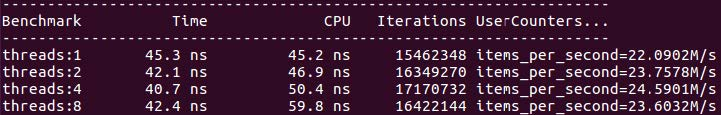
\includegraphics[width=0.9\textwidth]{content/2/chapter7/images/15.jpg}\\ 
图7.15 —— x86 CPU上无锁堆栈的性能(与图7.11相比)
\end{center}

为了进行比较,自旋锁保护的堆栈可以在同一台机器上每秒执行大约70M个操作。这与前一节对性能评估的预期一致。然而,同样的评估表明,无锁堆栈可能优于ARM处理器。基准测试证明了我们的努力没有白费:

%\hspace*{\fill} \\ %插入空行
\begin{center}
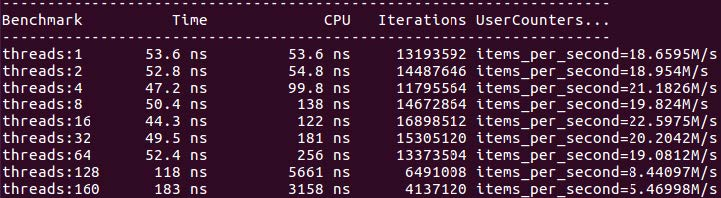
\includegraphics[width=0.9\textwidth]{content/2/chapter7/images/16.jpg}\\ 
图7.16 - ARM CPU上无锁堆栈的性能(与图7.12相比)
\end{center}

基于锁的堆栈单线程性能更好,如果线程数量大,则无锁堆栈的速度要快得多。如果基准测试包含大量的\texttt{top()}调用(许多线程在一个线程抛出顶层元素之前读取了它),或者如果生产者和消费者线程是不同的(一些线程只使用\texttt{push()},而其他线程只使用\texttt{pop()}),那么无锁堆栈的优势就会更大。

本节中,我们研究了线程安全堆栈数据结构的不同实现。为了理解线程安全需要什么,必须分别分析每个操作,以及多个并发操作的交互。以下是我们得到的经验:

\begin{itemize}
\item 
有了好的锁实现,锁保护的堆栈提供了合理的性能,并且比其他选择简单得多。

\item 
关于数据结构的使用,限制特定于应用程序的信息,都应该用来以较低的成本获得较好的性能。但这不是开发通用解决方案的地方,而实现尽可能少的特性,并试图从限制中获得性能优势才是要做的事情。

\item 
通用的无锁实现是可能的,但对于像堆栈这样简单的数据结构,也相当复杂。有时,这种复杂性甚至是合理的。

\end{itemize}

目前为止,我们还没有讨论到内存管理的问题。当堆栈耗尽容量时,它隐藏在分配更多内存的后面。我们稍后会再回到这个问题上的。这里,先让我们探索一下其他的数据结构。


































